\chapter{Sekwencjonowanie i adnotacja genomu}
\label{section:biologiny_wstep}

\section{Sekwencjonowanie i asembling DNA}
Sekwencjonowanie to jedna z technik biologii molekularnej, pozwalająca na odczytanie kolejności nukleotydów w cząsteczce DNA.

Najlepiej byłoby, gdyby projekt genomu reprezentował kompletną sekwencję nukleotydową wszystkich chromosomów danego gatunku. 
Jednak w rzeczywistości, istnieje wiele potencjalnych problemów związanych z procesem sekwencjonowania. Nie istnieje bowiem, jedna, prawdziwa sekwencja dla gatunku z powodu indywidualnej zmienności genetycznej jednostek. 
Nawet komórki tego samego osobnika mogą różnić się w zawartości genetycznej z powodu mutacji somatycznych. Złożony genom będzie tylko jedną reprezentacją wariacji występującej u danego gatunku. 
Zasadniczo sekwencjonuje się tylko jednego osobnika, ale czasami genom stanowi konsensus wielu połączonych próbek (projekt HUGO). 
Należy zdawać sobie sprawę, że procesowi sekwencjonowania zawsze będą towarzyszyć błędy na poziomie poszczególnych nukleotydów oraz ich kolejności (błędy montażu). 
Każdy złożony genom jest wynikiem serii złożeń metodami heurystycznymi i powinien być traktowany jako robocza hipoteza.

\begin{figure}[h]
	\centering
	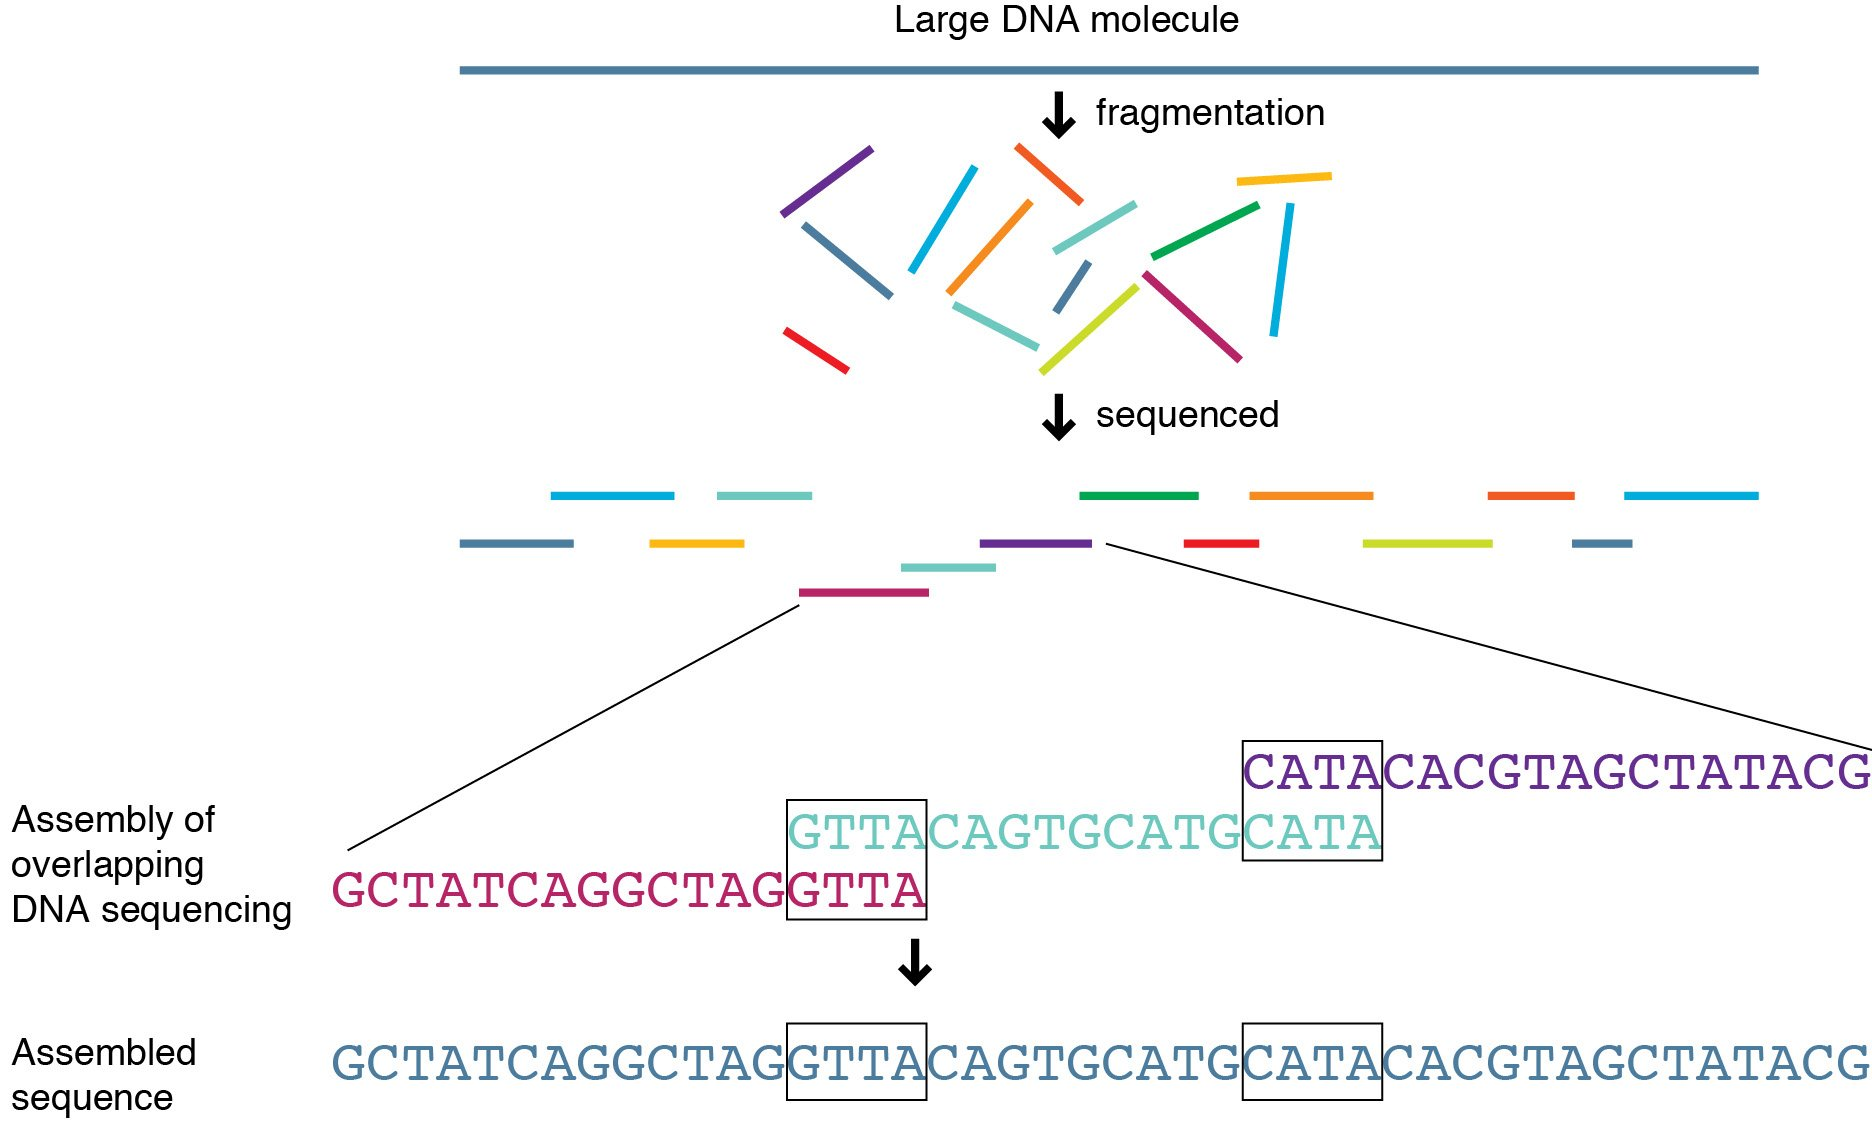
\includegraphics[width=0.9\textwidth]{img/sequenctioning-process.png}
	%zdjecie z %http://knowgenetics.org/whole-genome-sequencing/
	\caption{Schemat sekwencjonowania}
	\vspace{-0.5cm}
	\caption*{\scriptsize Źródło: \url{http://knowgenetics.org/whole-genome-sequencing/}}
	\label{img:schemat-sekwencjonowania}
\end{figure}

Większość projektów, w początkowej fazie sekwencjonowania kieruje się strategią polegającą na losowym pocięciu DNA na bardzo małe fragmenty.
W zależności od wykorzystanej technologii, fragmenty mogą mieć różne długości. Istnieje trend w kierunku przeprowadzania odczytów technikami dającymi coraz krótsze fragmenty. 
Tradycyjne sposoby (Sanger) dawały fragmenty długości około 1000 par zasad. Obecnie wykorzystywane techniki dające najkrótsze rezultaty osiągają wyniki rzędu dziesiątek pz. (SOLiD, Illumina - rys.\ref{img:sekwencjoner-illumina}).

\begin{figure}[h]
	\centering
	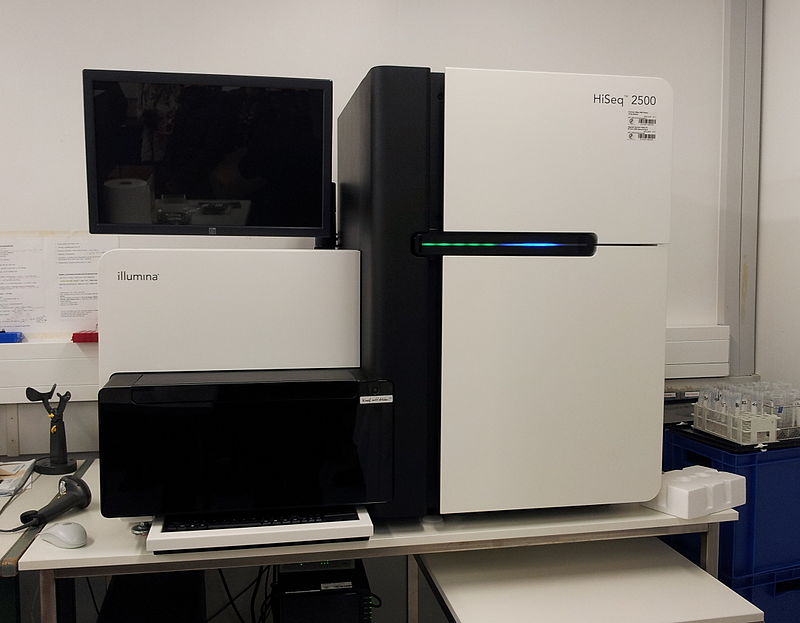
\includegraphics[width=0.75\textwidth]{img/sekwencjoner-illumina.jpg}
	%zdjecie z http://wiedza.alkahest.umcs.pl/jak-limfocyty-t-przekazuja-informacje/
	\caption{Sekwencjoner Illumina HiSeq 2500}
	\vspace{-0.5cm}
	\caption*{\scriptsize Źródło: \url{http://wiedza.alkahest.umcs.pl/jak-limfocyty-t-przekazuja-informacje/}}
	\label{img:sekwencjoner-illumina}
\end{figure}

Następie, w procesie asemblingu, fragmenty sekwencji są składane w dłuższe odcinki. Dobór algorytmu jest zależny od długości odcinków zsekwencjonowanych w poprzednim etapie. Jest to proces skomplikowany i wykorzystywane są do tego zasobożerne programy. 
Efektem początkowego składania sekwencji są kontigi.
Na dalszych etapach, po analizach wykorzystujących biblioteki dłużych sekwencji DNA, kontigi są zespalane w struktury zwane skafoldami.
Mają one zazwyczaj postać sekwencji z lukami o znanej długości - dziury oznaczane są znakiem "N".

\section{Adnotacje}

\section{Prezentacja danych}

\section{Przegląd literatury}

\chapter{Bioinformatyka w praktyce}

\section{Medycyna}
Posiadamy aktualnie techniczne możliwości aby stosować indywidualną wiedzę o indywidualnym genomie człowieka do projektowania indywidualnego leczenia. Dzięki medycynie spersonalizowanej jesteśmy w stanie w wielu przypadkach przewidywać ryzyko zachorowania na daną chorobę. Analizując genom, możemy zidentyfikować mutacje, które powodują, że niektóre białka działają w sposób inny niż powinny. Wykrycie takich przypadków nie oznacza, że człowiek od razu zachoruje, ponieważ istnieje bardzo rozbudowana sieć zależności i jeżeli jedno białko nie działa to być może w ten sam sposób funkcjonuje inne. Ma to natomiast istotne znaczenie przy projektowaniu leczenia. W sytuacji gdy dane białko nie działa, a standardowo leczymy chorobę modyfikując to białko, nabywamy cenną informacje, że leczenie należy przeprowadzić w inny sposób. Dążymy do tego aby minimalizować koszt i czas leczenia pacjentów, oraz zwiększyć wykrywalność chorób.

%\subsection{Farmaceutyka}
%\subsection{Kryminalistyka}
%\subsection{Sądownictwo}
%\subsection{Rolnictwo}
%\subsection{Archeologia}

%\section{Bioinformatyka w ujęciu algorytmicznym}
%\subsection{Bazy danych}
%\subsection{big data}
%\subsection{uczenie maszynowe}
%\subsection{metody optymalizacji}
%\subsection{teoria grafów}

\section{Problemy bioinformatyki}
Bioinformatyka, jak każda dziedzina naukowa boryka się z pewnymi problemami. Problem dotyczący baz danych polega na tym, że wiele baz powstaje i często potem nic się z nimi nie dzieje. Z każdym dniem poznajemy tysiące nowych sekwencji, które są deponowane w cyfrowych przechowalniach. Te podstawowe bazy są utrzymywane i z powodzeniem wykorzystywane do naukowych doświadczeń, jednakże problemem są bazy wtórne, bazujące na wynikach z wcześniejszych, podstawowych eksperymentów. Gromadzą one najczęściej zbiór informacji pochodzący z różnych miejsc i często są one po stosunkowo niedługim czasie nieaktualne.

Projekty bioinformatyczne często zostają zakończone opracowaniem bazy danych, po czym finansowanie projektu kończy się, projekt nie jest kontynuowany.
Jako, że mamy do czynienia z danymi biologicznymi oznacza to, że eksperymenty zazwyczaj obarczone są jakimś ryzykiem błędu. Niejednokrotnie zdarza się, że do bazy pierwotnej są wprowadzane modyfikacje, które nie zostają już uwzględnione w późniejszych bazach wtórnych. Błędy te propagują się na następne projekty. W~przypadku zakończenia projektu bazy wtórnej, pomimo aktualizacji danych pierwotnych, na których się opierała, informacje wtórne nie zostają już zmienione. Jest to dość poważny problem z jakim obecnie świat bioinformatyki boryka się.

Wspomniane zbiory danych często są ogromne. Sekwencja przykładowego genomu człowieka zajmuje ponad 3GB, natomiast opis samego eksperymentu sekwencjonowania może zająć nawet kilkaset gigabajtów. Pojawiający się problem jest natury technicznej - chodzi o sposób przechowywania danych. Okazuje się, że często bardziej opłaca się laboratorium ponownie przeprowadzić eksperyment sekwencjonowania, niż przechowywać wyniki doświadczeń na dyskach, gdyż jest to zbyt kosztowne. 

Kolejnym problemem jest mnogość standardów. Często gdy jest jakiś problem, rozwiązanie projektowane jest od podstaw. Takie podejście skutkuje tym, że dla pojedynczego zadania, mamy kilkanaście bądź kilkadziesiąt różnych metod, które nie koniecznie są ze sobą kompatybilne. Jednym z głównych problemów, z jakim zmagają się biolodzy przy analizie danych jest to, że wyjście z jednego programu nie jest kompatybilne z wejściem drugiego programu, który potrzebują aktualnie wykorzystać. Próby rozwiązania takiego kłopotu skutkują często zdefiniowaniem kolejnego standardu, co może jeszcze bardziej skomplikować sytuację jeśli nowy sposób się nie zostanie przyjęty przez większe grono naukowców.


%-niekontynuowane projekty \\
%-dane bazują na eksperymentach, błędy propagujące się \\
%-wiele różnych standardów, niekompatybilne \\
%-nieinformatyczni biolodzy \\
%-sposoby finansowania nauki \\

\section{Centralny dogmat bioinformatyki}
Podstawowym założeniem w bioinformatyce jest następująca zależność:
Informacja, która jest zawarta w sekwencji nukleotydowej bezpośrednio przekłada się na strukturę przestrzenną białek i innych cząsteczek, które są w genomie zakodowane. Dzięki strukturze przestrzennej, białka mogą na siebie bezpośrednio oddziaływać, co oznacza że pełnią one pewne funkcje biochemiczne. Funkcją biochemiczną może być np. reakcja w którą wchodzi dane białko łącząc się z inną substancją. Efekt końcowy oddziaływań zbioru wybranych białek obserwujemy w postaci np. wyglądu zewnętrznego, zachowania, funkcjonowania organizmu.

Informacje sekwencyjne jesteśmy w stanie eksperymentalnie pozyskać bardzo łatwo. Trudniej jest określić struktury przestrzenne i funkcje biochemiczne jakie pełnią.
Obecnie nacisk jest wywierany na ustalenie procesu w jaki sposób na podstawie sekwencji możemy określić strukturę przestrzenną bądź później, funkcję danego związku chemicznego.
Z samej obserwacji fenotypu nic nie wynosimy. Dążymy do tego aby dowiedzieć się jakie konkretne białka odpowiadają za dany fenotyp. Chcemy posiąść kompletną wiedzę na temat funkcjonowania organizmu. Kryje się za tym znajomość wszystkich genów jakie mogą w tym organiźmie występować, odmian, mutacji i ch wzajemnych wpływów.

[RYSUNEK sekwencja -> struktura -> funkcja biochemiczna -> fenotyp]

%-dna, rna, białko \\
%-informacja genetyczna \\
%-struktura molekularna \\
%-funkcja biochemiczna \\
%-fenotyp

%\section{Rozwój bioinformatyki}
%\subsection{wcześniej}
%\subsection{obecnie}
%\subsection{w przyszłości}

\section{Genom ogórka}
-sggw
